\documentclass[paper=a4, fontsize=11pt]{scrartcl} 

\usepackage[T1]{fontenc} 
\usepackage[english]{babel}
\usepackage{amsmath,amsfonts,amsthm}

\usepackage{lipsum}

\usepackage{graphicx}
\usepackage{float}
  \floatplacement{figure}{H}
  \floatplacement{table}{H}
  
\usepackage{sectsty} 
\allsectionsfont{\centering \normalfont\scshape} 

\usepackage{fancyhdr} % Custom headers and footers
\pagestyle{fancyplain} % Makes all pages in the document conform to the custom headers and footers
\fancyhead{} % No page header - if you want one, create it in the same way as the footers below
\fancyfoot[L]{} % Empty left footer
\fancyfoot[C]{} % Empty center footer
\fancyfoot[R]{\thepage} % Page numbering for right footer
\renewcommand{\headrulewidth}{0pt} % Remove header underlines
\renewcommand{\footrulewidth}{0pt} % Remove footer underlines
\setlength{\headheight}{13.6pt} % Customize the height of the header

\usepackage[labelformat=empty]{caption}
\usepackage{color}
\usepackage{listings}
\lstset{ %
language=bash,                % choose the language of the code
basicstyle=\footnotesize,       % the size of the fonts that are used for the code
numbers=left,                   % where to put the line-numbers
numberstyle=\footnotesize,      % the size of the fonts that are used for the line-numbers
stepnumber=1,                   % the step between two line-numbers. If it is 1 each line will be numbered
numbersep=5pt,                  % how far the line-numbers are from the code
backgroundcolor=\color{white},  % choose the background color. You must add \usepackage{color}
showspaces=false,               % show spaces adding particular underscores
showstringspaces=false,         % underline spaces within strings
showtabs=false,                 % show tabs within strings adding particular underscores
frame=single,           % adds a frame around the code
tabsize=2,          % sets default tabsize to 2 spaces
captionpos=b,           % sets the caption-position to bottom
breaklines=true,        % sets automatic line breaking
breakatwhitespace=false,    % sets if automatic breaks should only happen at whitespace
escapeinside={\%*}{*)}          % if you want to add a comment within your code
}
\usepackage{hyperref}


\numberwithin{equation}{section} % Number equations within sections (i.e. 1.1, 1.2, 2.1, 2.2 instead of 1, 2, 3, 4)
\numberwithin{figure}{section} % Number figures within sections (i.e. 1.1, 1.2, 2.1, 2.2 instead of 1, 2, 3, 4)
\numberwithin{table}{section} % Number tables within sections (i.e. 1.1, 1.2, 2.1, 2.2 instead of 1, 2, 3, 4)

\setlength\parindent{0pt} % Removes all indentation from paragraphs - comment this line for an assignment with lots of text

%----------------------------------------------------------------------------------------
%	TITLE SECTION
%----------------------------------------------------------------------------------------

\newcommand{\horrule}[1]{\rule{\linewidth}{#1}} % Create horizontal rule command with 1 argument of height

\title{	
\normalfont \normalsize 
\textsc{Computational Science - ITB} \\ [25pt] % Your university, school and/or department name(s)
\horrule{0.5pt} \\[0.4cm] % Thin top horizontal rule
\small  Pengenalan Sains Komputasi - Movement of Ants\\ % The assignment title
%\horrule{2pt} \\[0.5cm] % Thick bottom horizontal rule
}

\author{\small{Ridlo W. Wibowo || 20912009}} % Your name

\date{\normalsize\today} % Today's date or a custom date

\begin{document}

\maketitle % Print the title

\large \textbf{Problem.}\\
Apply the model of ant movement in a 17 $\times$ 17 grid where there are 20 ant's initially located randomly. Assume that there is food right in the middle of the grid, in which the initial amount of chemical is 10, where in the other cells, the amount is 0. Run the program 5 times, each for t=10, t=20, ... , t=100, and write your conclusion of the simulation.\\

\vspace{1cm}
\large \textbf{Documentation.}\\
Dengan hanya menggunakan asumsi adanya pheromon sebagai 'petunjuk arah' bagi semut, dan apabila yang dicek adalah untuk semua arah, maka yang akan terjadi adalah semut akan bolak-balik di tempat yang sama.
Oleh karena itu dilakukan sedikit perubahan dalam membuat simulasi ini, yaitu:
\begin{itemize}
\item simulasi melibatkan 8 arah.
\item semut hanya memeriksa keberadaan pheromon di 5 grid  di arah dimana ia menghadap (depan dan samping) dari 8 grid tersebut.
\item semut sebagai objek (bukan cellular automaton), sehingga diperbolehkan semut berada pada grid yang sama, dan pada simulasi kali ini diasumsikan tidak terjadi tumbukan.
\item periodic boundary
\item ada 3 makanan di tengah (dengan menganggap pheromon tetap selama iterasi)
\item terdapat \textit{probabilitas semut bosan} untuk mengurangi peluang semut berputar pada kumpulan grid dan memperbesar peluang semut sampai di makanan (dalam simulasi ini saya ambil 0.1).
\item penambahan pheromon setelah grid ditempati semut dan pengurangan pheromon setiap waktu dilakukan secara linear menggunakan bilangan bulat saja.
\end{itemize}

Menggunakan beberapa asumsi di atas lalu dibuat simulasi sederhana tersebut, menggunakan \textit{C++} dan \textit{OpenGL}. Warna kuning menunjukkan grid tempat semut, semakin putih semakin banyak pheromonnya.
Tiga grid putih ditengah merupakan makanan, dan semut disimbolkan dengan grid merah. Karena keterbatasan waktu kode masih kurang terstruktur dengan baik, dan banyak penggunaan \textit{IF} yang seharusnya dapat dihindari (program terlampir).\\

\textit{Screenshot} setelah cukup stabil:
\begin{figure}
	\centering
	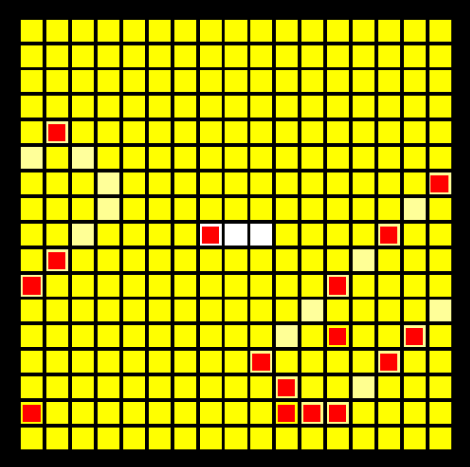
\includegraphics[width=0.45\textwidth]{semut.png}
	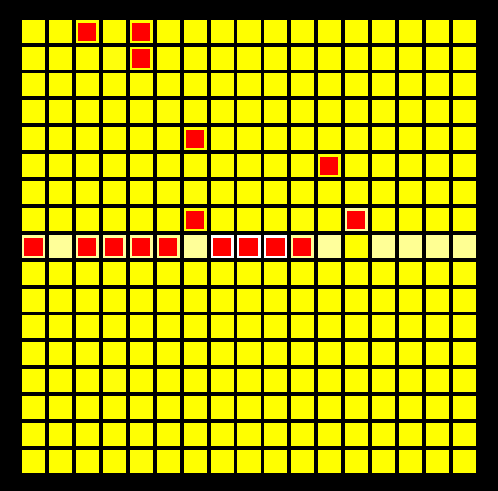
\includegraphics[width=0.45\textwidth]{semut2.png}
\end{figure}
\begin{figure}
	\centering
	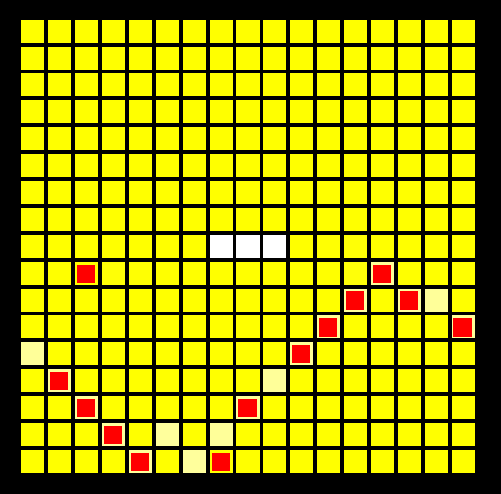
\includegraphics[width=0.45\textwidth]{semut3.png}
	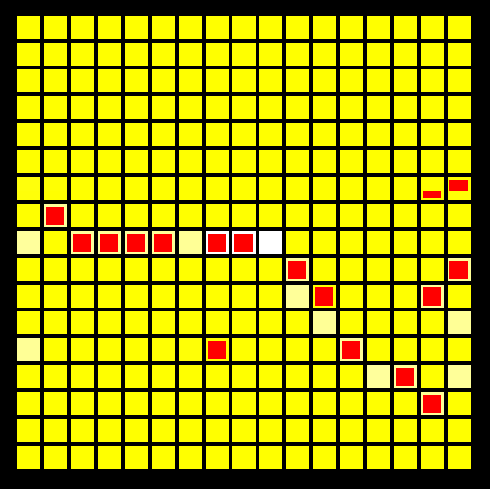
\includegraphics[width=0.45\textwidth]{semut4.png}
\end{figure}
\begin{figure}
	\centering
	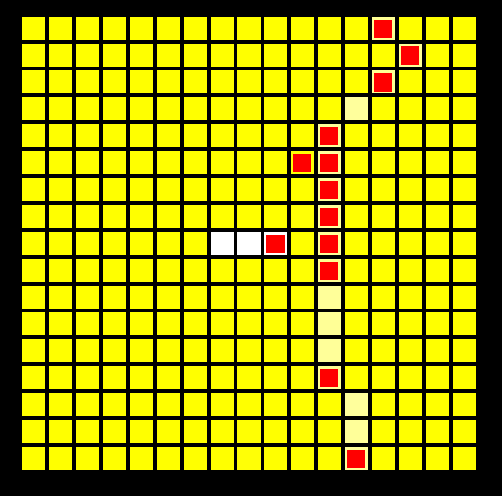
\includegraphics[width=0.45\textwidth]{semut5.png}
	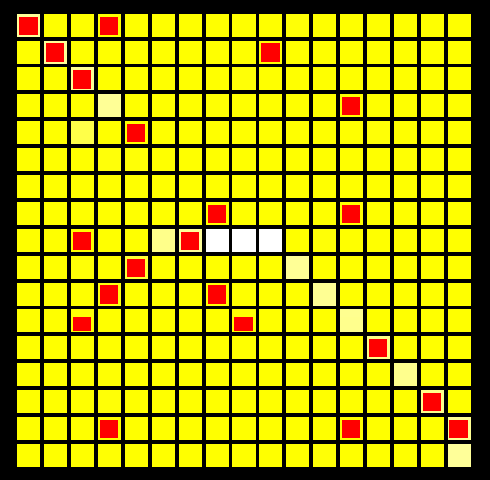
\includegraphics[width=0.45\textwidth]{semut6.png}
	\caption{Screenshot kondisi setelah cukup stabil. Kotak kuning sebagai grid, semakin putih warnanya semakin banyak jumlah pheromon, tiga kotak putih ditengah merupakan grid yang dibuat konstan jumlah pheromonnya, sedangkan gird merah melambangkan posisi semut.}
\end{figure}

cuplikan animasi dapat dilihat di \url{http://www.youtube.com/watch?v=DWg_oeGBZp4/}

\vspace{1cm}
\textbf{Diskusi}
\begin{enumerate}
\item semakin lama waktu iterasi maka semut akan cenderung berkumpul atau membuat suatu jalur.
\item untuk membuat simulasi lebih real sepertinya dapat dilakukan dengan menggunakan dua tipe pheromon yakni pheromon makanan dan pheromon rumah, dan semut berasal dari suatu tempat yang sama (koloni).
\item dalam kondisi nyata memang cenderung tidak ada semut yang balik arah.
\item perlu pemodelan penambahan dan pengurangan jumlah pheromon yang lebih baik (dalam program ini pheromon hanya berupa bilangan integer, dan bertambah/berkurang secara linear saja). 
\end{enumerate}

\vspace{1.5cm}
\textit{\textbf{Program}}
\lstset{frameround=fttt}
\begin{lstlisting}
// Copyleft (c) Ridlo W. Wibowo
// Simut
#include <iostream>
#include <stdlib.h>
#include <GL/gl.h>
#include <GL/glut.h>
#include <fstream>
#include <time.h>
#define MAX 17
#define maxSemut 20
using namespace std;

int grid [MAX][MAX];
int grid2[MAX][MAX];
int strong[MAX][MAX];
bool f = false;
int tpm = 100;
double boredProb = 0.1;
int maxPher = 200;
/* N  = 0, NE = 1, E  = 2, SE = 3, S  = 4, SW = 5, W  = 6, NW = 7 */

double unirand(){ return (double)rand()/(double)RAND_MAX;}

int getStrong(int x, int y, int direc){ 
    int m = x+MAX; int n = y+MAX; int kuat=0; int arahbaru = direc;
    if (direc == 0){ 
            if (grid[m%MAX][(n+1)%MAX] > kuat){kuat = grid[m%MAX][(n+1)%MAX]; arahbaru=0;}
            if (grid[(m-1)%MAX][n%MAX] > kuat){ kuat = grid[(m-1)%MAX][n%MAX] ; arahbaru = 6;}
            if (grid[(m-1)%MAX][(n+1)%MAX] > kuat){ kuat = grid[(m-1)%MAX][(n+1)%MAX] ; arahbaru = 7;}
            if (grid[(m+1)%MAX][(n+1)%MAX] > kuat){ kuat = grid[(m+1)%MAX][(n+1)%MAX] ; arahbaru = 1;}
            if (grid[(m+1)%MAX][n%MAX] > kuat){ kuat = grid[(m+1)%MAX][n%MAX] ; arahbaru = 2;}
    }
    if (direc == 1){
            if (grid[m%MAX][(n+1)%MAX] > kuat){kuat = grid[m%MAX][(n+1)%MAX]; arahbaru = 0;}
            if (grid[(m+1)%MAX][(n+1)%MAX] > kuat){ kuat = grid[(m+1)%MAX][(n+1)%MAX] ; arahbaru = 1;}
            if (grid[(m-1)%MAX][(n+1)%MAX] > kuat){ kuat = grid[(m-1)%MAX][(n+1)%MAX] ; arahbaru = 7;}
            if (grid[(m+1)%MAX][n%MAX] > kuat){ kuat = grid[(m+1)%MAX][n%MAX] ; arahbaru = 2;}
            if (grid[(m+1)%MAX][(n-1)%MAX] > kuat){ kuat = grid[(m+1)%MAX][(n-1)%MAX] ; arahbaru = 3;}
    }
    if (direc == 2){
            if (grid[m%MAX][(n+1)%MAX] > kuat){kuat = grid[m%MAX][(n+1)%MAX]; arahbaru = 0;}
            if (grid[(m+1)%MAX][(n+1)%MAX] > kuat){ kuat = grid[(m+1)%MAX][(n+1)%MAX] ; arahbaru = 1;}
            if (grid[(m+1)%MAX][n%MAX] > kuat){ kuat = grid[(m+1)%MAX][n%MAX] ; arahbaru = 2;}
            if (grid[(m+1)%MAX][(n-1)%MAX] > kuat){ kuat = grid[(m+1)%MAX][(n-1)%MAX] ; arahbaru = 3;}
            if (grid[m%MAX][(n-1)%MAX] > kuat){ kuat = grid[m%MAX][(n-1)%MAX] ; arahbaru = 4;}
    }
    if (direc == 3){
            if (grid[(m+1)%MAX][(n+1)%MAX] > kuat){ kuat = grid[(m+1)%MAX][(n+1)%MAX] ; arahbaru = 1;}
            if (grid[(m+1)%MAX][n%MAX] > kuat){ kuat = grid[(m+1)%MAX][n%MAX] ; arahbaru = 2;}
            if (grid[(m+1)%MAX][(n-1)%MAX] > kuat){ kuat = grid[(m+1)%MAX][(n-1)%MAX] ; arahbaru = 3;}
            if (grid[m%MAX][(n-1)%MAX] > kuat){ kuat = grid[m%MAX][(n-1)%MAX] ; arahbaru = 4;}
            if (grid[(m-1)%MAX][(n-1)%MAX] > kuat){ kuat = grid[(m-1)%MAX][(n-1)%MAX] ; arahbaru = 5;}
    }
    if (direc == 4){
            if (grid[(m+1)%MAX][n%MAX] > kuat){ kuat = grid[(m+1)%MAX][n%MAX] ; arahbaru = 2;}
            if (grid[(m+1)%MAX][(n-1)%MAX] > kuat){ kuat = grid[(m+1)%MAX][(n-1)%MAX] ; arahbaru = 3;}
            if (grid[m%MAX][(n-1)%MAX] > kuat){ kuat = grid[m%MAX][(n-1)%MAX] ; arahbaru = 4;}
            if (grid[(m-1)%MAX][(n-1)%MAX] > kuat){ kuat = grid[(m-1)%MAX][(n-1)%MAX] ; arahbaru = 5;}
            if (grid[(m-1)%MAX][n%MAX] > kuat){ kuat = grid[(m-1)%MAX][n%MAX] ; arahbaru = 6;}
    }
    if (direc == 5){
            if (grid[(m+1)%MAX][(n-1)%MAX] > kuat){ kuat = grid[(m+1)%MAX][(n-1)%MAX] ; arahbaru = 3;}
            if (grid[m%MAX][(n-1)%MAX] > kuat){ kuat = grid[m%MAX][(n-1)%MAX] ; arahbaru = 4;}
            if (grid[(m-1)%MAX][(n-1)%MAX] > kuat){ kuat = grid[(m-1)%MAX][(n-1)%MAX] ; arahbaru = 5;}
            if (grid[(m-1)%MAX][n%MAX] > kuat){ kuat = grid[(m-1)%MAX][n%MAX] ; arahbaru = 6;}
            if (grid[(m-1)%MAX][(n+1)%MAX] > kuat){ kuat = grid[(m-1)%MAX][(n+1)%MAX] ; arahbaru = 7;}
    }
    if (direc == 6){
            if (grid[m%MAX][(n-1)%MAX] > kuat){ kuat = grid[m%MAX][(n-1)%MAX] ; arahbaru = 4;}
            if (grid[(m-1)%MAX][(n-1)%MAX] > kuat){ kuat = grid[(m-1)%MAX][(n-1)%MAX] ; arahbaru = 5;}
            if (grid[(m-1)%MAX][n%MAX] > kuat){ kuat = grid[(m-1)%MAX][n%MAX] ; arahbaru = 6;}
            if (grid[(m-1)%MAX][(n+1)%MAX] > kuat){ kuat = grid[(m-1)%MAX][(n+1)%MAX] ; arahbaru = 7;}
            if (grid[m%MAX][(n+1)%MAX] > kuat){kuat = grid[m%MAX][(n+1)%MAX]; arahbaru = 0;}
    }
    if (direc == 7){
            if (grid[(m-1)%MAX][(n-1)%MAX] > kuat){ kuat = grid[(m-1)%MAX][(n-1)%MAX] ; arahbaru = 5;}
            if (grid[(m-1)%MAX][n%MAX] > kuat){ kuat = grid[(m-1)%MAX][n%MAX] ; arahbaru = 6;}
            if (grid[(m-1)%MAX][(n+1)%MAX] > kuat){ kuat = grid[(m-1)%MAX][(n+1)%MAX] ; arahbaru = 7;}
            if (grid[m%MAX][(n+1)%MAX] > kuat){kuat = grid[m%MAX][(n+1)%MAX]; arahbaru = 0;}
            if (grid[(m+1)%MAX][(n+1)%MAX] > kuat){ kuat = grid[(m+1)%MAX][(n+1)%MAX] ; arahbaru = 1;}
    }
    
    return arahbaru;
    /*
    for (int i=0;i<MAX;i++){
        for (int j=0;j<MAX;j++){
            int m = i + MAX; int n = j + MAX; int kuat=0; //strong[i][j] = 0;
            if (grid[m%MAX][(n+1)%MAX] > kuat){kuat = grid[m%MAX][(n+1)%MAX]; strong[i][j] = 0;}
            if (grid[(m+1)%MAX][(n+1)%MAX] > kuat){ kuat = grid[(m+1)%MAX][(n+1)%MAX] ; strong[i][j] = 1;}
            if (grid[(m+1)%MAX][n%MAX] > kuat){ kuat = grid[(m+1)%MAX][n%MAX] ; strong[i][j] = 2;}
            if (grid[(m+1)%MAX][(n-1)%MAX] > kuat){ kuat = grid[(m+1)%MAX][(n-1)%MAX] ; strong[i][j] = 3;}
            if (grid[m%MAX][(n-1)%MAX] > kuat){ kuat = grid[m%MAX][(n-1)%MAX] ; strong[i][j] = 4;}
            if (grid[(m-1)%MAX][(n-1)%MAX] > kuat){ kuat = grid[(m-1)%MAX][(n-1)%MAX] ; strong[i][j] = 5;}
            if (grid[(m-1)%MAX][n%MAX] > kuat){ kuat = grid[(m-1)%MAX][n%MAX] ; strong[i][j] = 6;}
            if (grid[(m-1)%MAX][(n+1)%MAX] > kuat){ kuat = grid[(m-1)%MAX][(n+1)%MAX] ; strong[i][j] = 7;}
        }
    }
    */
    
}

class varSemut{
    public:
        int x, y, arah;
        void set_value(int, int, int);
        void sensing();
        void buangpher();
} semut[maxSemut];

void varSemut::set_value(int a, int b, int c){x = (a+MAX)%MAX; y = (b+MAX)%MAX; arah = c;}

void varSemut::buangpher(){
    if (grid2[x][y] < 50){
        grid2[x][y] = grid2[x][y] + 2;
    }
}

void varSemut::sensing(){
    int arahnew = getStrong(x, y, arah);
    if (arahnew == 0){ 
        x = x; 
        y = (y+MAX+1)%MAX;
        arah = arahnew;
    }
    if (arahnew == 1){ 
        x = (x+MAX+1)%MAX; 
        y = (y+MAX+1)%MAX;
        arah = arahnew;
    }
    if (arahnew == 2){ 
        x = (x+MAX+1)%MAX; 
        y = y;
        arah = arahnew;
    }
    if (arahnew == 3){ 
        x = (x+MAX+1)%MAX; 
        y = (y+MAX-1)%MAX;
        arah = arahnew;
    }
    if (arahnew == 4){ 
        x = x; 
        y = (y+MAX-1)%MAX;
        arah = arahnew;
    }
    if (arahnew == 5){ 
        x = (x+MAX-1)%MAX; 
        y = (y+MAX-1)%MAX;
        arah = arahnew;
    }
    if (arahnew == 6){ 
        x = (x+MAX-1)%MAX; 
        y = y;
        arah = arahnew;
    }
    if (arahnew == 7){ 
        x = (x+MAX-1)%MAX; 
        y = (y+MAX+1)%MAX;
        arah = arahnew;
    }
}

void inisiasi();

void menu(int t){
	tpm = t;
	glutPostRedisplay();
}

void copy(){
	for(int i = 0; i < MAX; i++){
		for(int j = 0; j < MAX; j++){
			grid[i][j] = grid2[i][j];}}
}

void mlaku(){
    for (int k=0;k<maxSemut;k++){
        if (unirand() > boredProb){
            semut[k].buangpher();
            semut[k].sensing();
        }
        else {
            semut[k].buangpher();
            semut[k].set_value(semut[k].x + (-1 + (rand()%3)), semut[k].y + (-1 + (rand()%3)), rand()%8); //semutnya bosen
        }
    }
}

void jalan(){
    for (int i=0;i<MAX;i++){
        for (int j=0;j<MAX;j++){
            if (grid[i][j] > 0){ grid2[i][j] -= 1;}
        }
    }
    grid2[8][8] = 100;
    grid2[8][7] = 100;
    grid2[8][9] = 100;
    //grid2[7][8] = 100;
    //grid2[9][8] = 100;
    mlaku();
    copy();
}

void par(float x1, float x2, float y1, float y2, int val){
    glColor3f(1.0, 1.0, (float)val/(float)maxPher);
	glBegin(GL_QUADS);
	glVertex3f(x1, y1, 0.0);
	glVertex3f(x2, y1, 0.0);
	glVertex3f(x2, y2, 0.0);
	glVertex3f(x1, y2, 0.0);
	glEnd();
}

void sem(float x1, float x2, float y1, float y2){
    glColor3f(1.0, 0.0, 0.0);
	glBegin(GL_QUADS);
	glVertex3f(x1, y1, 0.0);
	glVertex3f(x2, y1, 0.0);
	glVertex3f(x2, y2, 0.0);
	glVertex3f(x1, y2, 0.0);
	glEnd();
}

void display(void){
	glClear(GL_COLOR_BUFFER_BIT | GL_DEPTH_BUFFER_BIT);
	glMatrixMode(GL_MODELVIEW);
	glLoadIdentity();
	glTranslatef(0.0, 0.0, -22.0);
    for (int k=0;k<maxSemut;k++){
        sem(-6.0 + 0.7 * semut[k].y + 0.15,
            -6.0 + 0.7 * (semut[k].y + 1) - 0.075,
             6.0 - 0.7 * semut[k].x + 0.15,
             6.0 - 0.7 * (semut[k].x - 1) - 0.075);
    }
	for(int i = 0; i < MAX; i++){
		for(int j = 0; j < MAX; j++){
				par(-6.0 + 0.7 * j + 0.1,
					-6.0 + 0.7 * (j + 1),
					6.0 - 0.7 * i + 0.1,
					6.0 - 0.7 * (i - 1),
                    grid[i][j]);
		}
	}
	glutSwapBuffers();
}

void myIdleFunc(int a) {
	jalan();
	glutPostRedisplay();
	if(f) glutTimerFunc(tpm, myIdleFunc, 0);
}

void inisiasi(){
	for (int i=0;i<MAX;i++){
        for (int j=0;j<MAX;j++){
            grid2[i][j] = 0;
        }
    }
    grid2[8][8] = 100;
    grid2[8][7] = 100;
    grid2[8][9] = 100;
    //grid2[7][8] = 100;
    //grid2[9][8] = 100;
    copy();
    for (int k=0;k<maxSemut;k++){
        semut[k].set_value(rand()%MAX, rand()%MAX, rand()%8);
    }
}

void keyboard(unsigned char key, int x, int y){
	if(key == 27) {		
		exit(0);	
	}else if((char)key == 'a'){
		if(!f) glutTimerFunc(tpm, myIdleFunc, 0);
		f = true;
	}else if((char)key == 's'){
		jalan();
		glutPostRedisplay();
	}else if((char)key == 'd'){
		f = false;
	}else if((char)key == 'f'){
		inisiasi();
        f = false;
		glutPostRedisplay();
    }
}

void init(){
	glEnable(GL_DEPTH_TEST);
	glEnable(GL_COLOR_MATERIAL);
	glEnable(GL_LIGHTING);
	glEnable(GL_LIGHT0);
	glEnable(GL_NORMALIZE);
	glShadeModel(GL_SMOOTH);	
	glLoadIdentity ();
	glOrtho(-1.0, 1.0, -1.0, 1.0, -1.0, 1.0);
	GLfloat acolor[] = {1.4, 1.4, 1.4, 1.0};
	glLightModelfv(GL_LIGHT_MODEL_AMBIENT, acolor);
}

void Reshape(int w, int h){
    glViewport(0, 0, w, h);
    glMatrixMode(GL_PROJECTION); 
	glLoadIdentity();
	gluPerspective(45.0, (float)w/(float)h, 0.1, 200.0);
}

int main(int argc, char** argv){
	srand(time(NULL));
    inisiasi();
	glutInit(&argc,argv);
	glutInitDisplayMode ( GLUT_DOUBLE | GLUT_RGB | GLUT_DEPTH);
	glutInitWindowSize(700,700);
	glutInitWindowPosition(500,0);
	glutCreateWindow("Semut muutmuut");
	glutCreateMenu(menu);
	glutAddMenuEntry( "20",  20);
	glutAddMenuEntry( "40",  40);
	glutAddMenuEntry( "60",  60);
	glutAddMenuEntry("100", 100);
	glutAddMenuEntry("150", 150);
	glutAddMenuEntry("200", 200);
	glutAttachMenu(GLUT_RIGHT_BUTTON);
	init();
	glutReshapeFunc(Reshape);
	glutKeyboardFunc(keyboard);
	glutDisplayFunc(display);
	glutMainLoop();
	return 0;
}
\end{lstlisting}

\end{document}